\documentclass{article}

\pdfoutput=1

\usepackage[utf8]{inputenc}
\usepackage[T1]{fontenc}
\usepackage[english]{babel}
\usepackage{amsmath}
\usepackage{lmodern}
\usepackage{units}
\usepackage{siunitx}
\usepackage{icomma}
\usepackage{graphicx}
\usepackage{caption}
\usepackage{subcaption}
\usepackage{color}
\newcommand{\N}{\ensuremath{\mathbbm{N}}}
\newcommand{\Z}{\ensuremath{\mathbbm{Z}}}
\newcommand{\Q}{\ensuremath{\mathbbm{Q}}}
\newcommand{\R}{\ensuremath{\mathbbm{R}}}
\newcommand{\C}{\ensuremath{\mathbbm{C}}}
\newcommand{\rd}{\ensuremath{\mathrm{d}}}
\newcommand{\id}{\ensuremath{\,\rd}}
\usepackage{hyperref}
%\usepackage{a4wide} % puts the page numbering further down the page.
\usepackage{pdfpages}
\usepackage{epstopdf}
\DeclareGraphicsExtensions{.eps}

\title{Home Assigment Week 1}
\author{Marcus Malmquist, marmalm, 941022}
\date{\today}

\begin{document}
\maketitle

\section{Task 1}
The results presented in this report was calculated using a Python-script I wrote and plotted on a simplified Smith chart, which I also made. I also solved this task by hand using a printed Smith chart to verify the result.

\subsection{a}\label{sec:a}
The antenna impedance (normalized with $\SI{50}{\ohm}$) can be seen in Figure~\ref{fig:smith1}. The antenna impedance for the frequency range $\SI{900}{\mega\hertz}$ to $\SI{3.6}{\giga\hertz}$ can be seen in Figure~\ref{fig:imp1}.
\begin{figure}
  \centering
  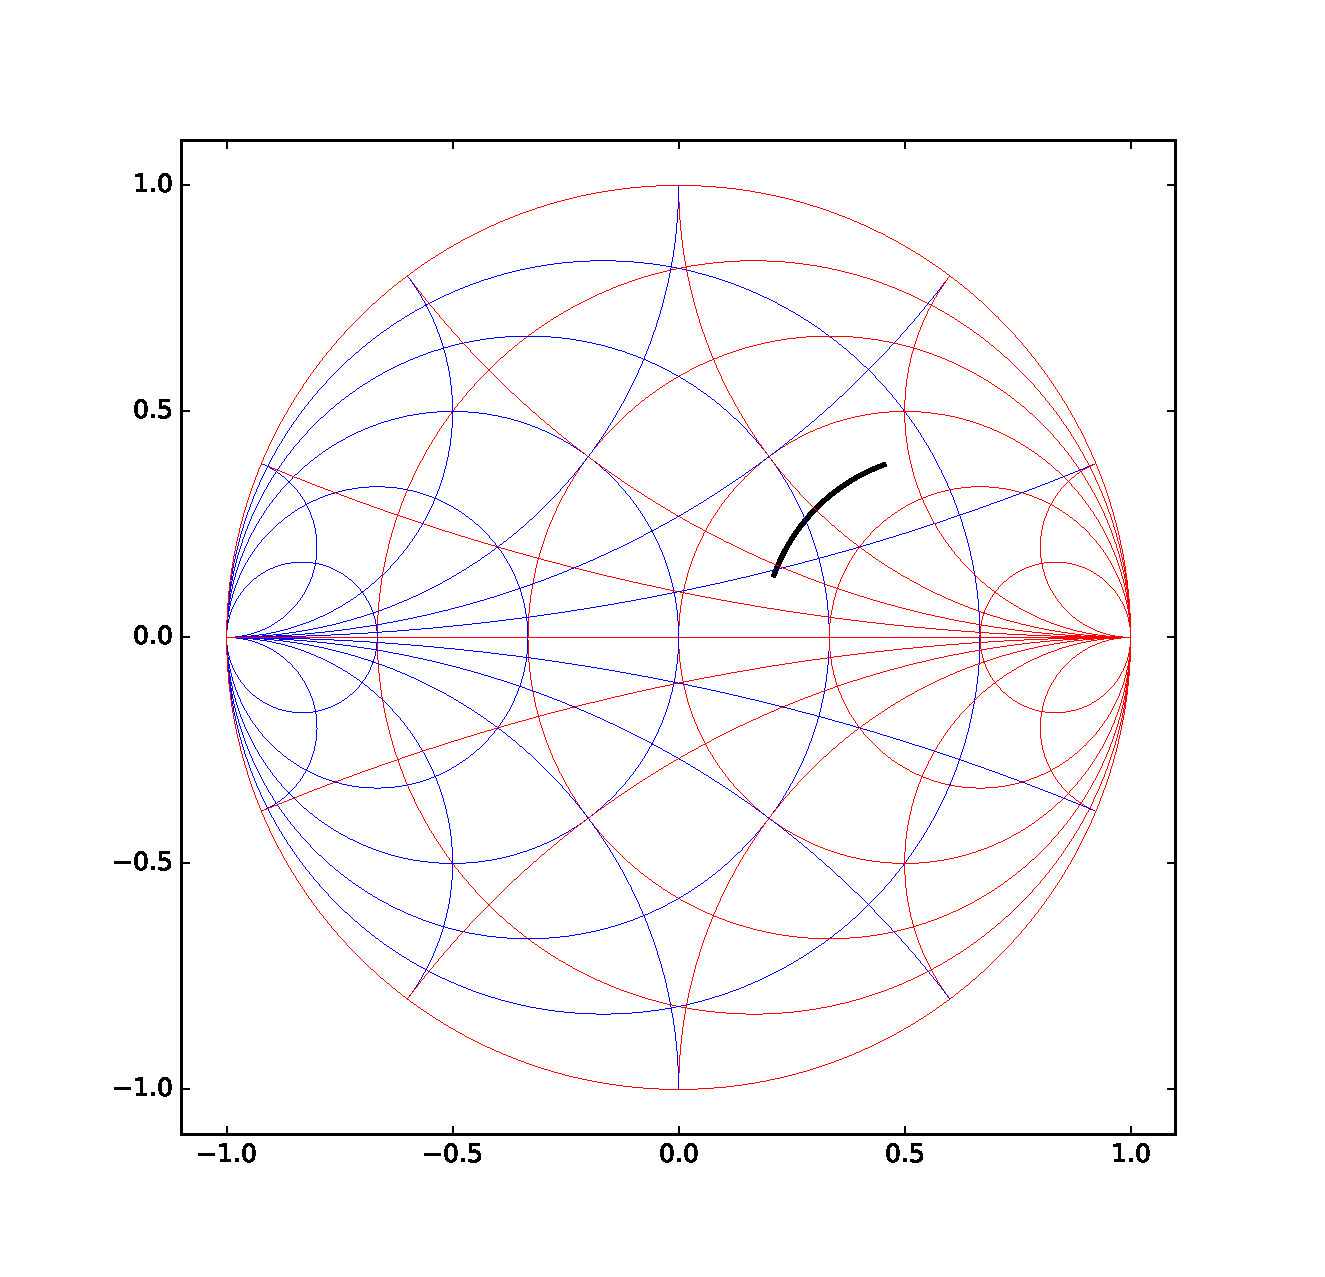
\includegraphics[width=\textwidth]{SmithChart1.eps}
  \caption{The figure shows the imput impedance of the antenna from Section~\ref{sec:a} normalized by $\SI{50}{\ohm}$ in the frequency range $\SI{900}{\mega\hertz}$ to $\SI{3.6}{\giga\hertz}$ in a Smith chart.}
  \label{fig:smith1}
\end{figure}
\begin{figure}
  \centering
  \includegraphics[width=\textwidth]{impedance1.eps}
  \caption{The figure shows the imput impedance of the antenna from Section~\ref{sec:a} in the frequency range $\SI{900}{\mega\hertz}$ to $\SI{3.6}{\giga\hertz}$. The horizontal axis shows the real part of the antenna impedance ($\Re\{Z_{\text{antenna}}\}$) and the vertical axis shows the imaginary part of the antenna impedance ($\Im\{Z_{\text{antenna}}\}$).}
  \label{fig:imp1}
\end{figure}

\subsection{b}\label{sec:b}
The return loss and VSWR can be seen in Figure~\ref{fig:ans1}.
\begin{figure}
  \centering
  \includegraphics[width=\textwidth]{Answers1.eps}
  \caption{The figure shows the return loss (left) and the standing wave ratio (right) for the antenna from Section~\ref{sec:b} in the frequency range $\SI{900}{\mega\hertz}$ to $\SI{3.6}{\giga\hertz}$.}
  \label{fig:ans1}
\end{figure}

\subsection{c}\label{sec:c}
The antenna impedance can be seen in Figure~\ref{fig:smith1}. The black dashed lines are normalized with $\SI{70}{\ohm}$ and represents intermediate impedances while the solid line is normalized with $\SI{50}{\ohm}$ and represents the antenna impedance normalized with the system impedance. The dotted lines represent how the end points of the impedance (i.e. the points where $f=\SI{900}{\mega\hertz}$ and $f=\SI{3.6}{\giga\hertz}$) moves in the smith chart. The antenna impedance for this frequency range can be seen in Figure~\ref{fig:imp2}.
\begin{figure}
  \centering
  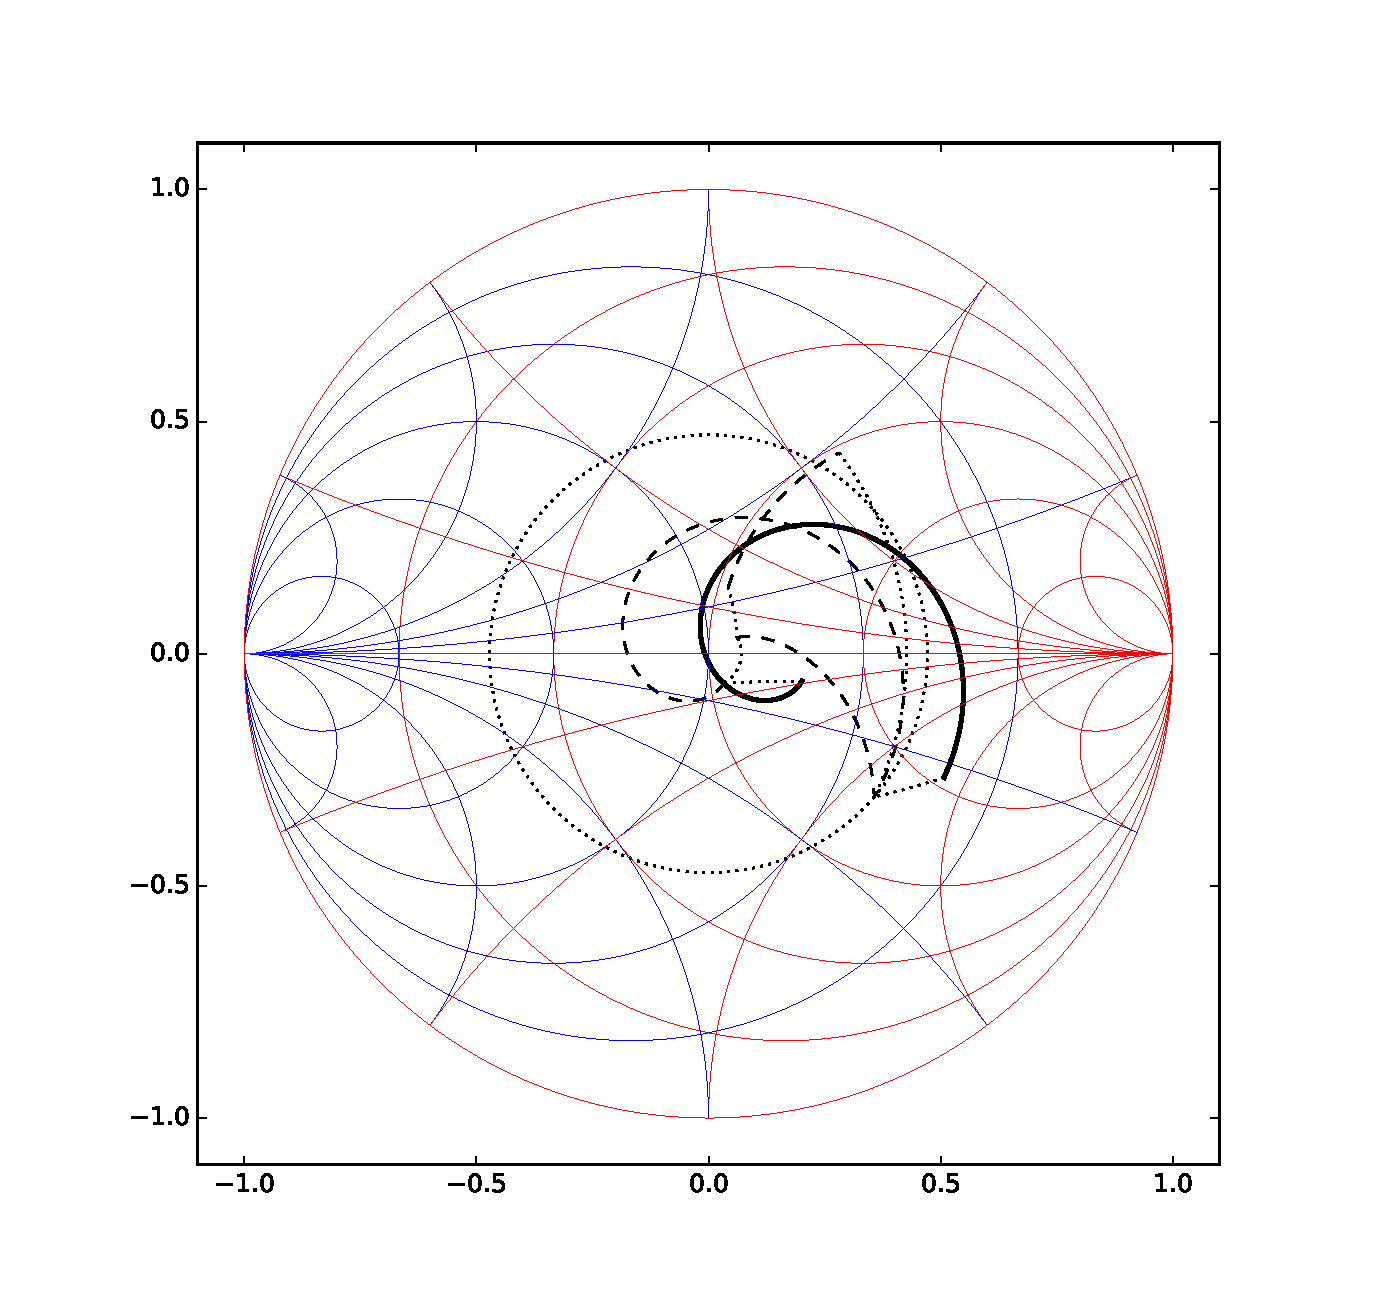
\includegraphics[width=\textwidth]{SmithChart2.eps}
  \caption{The figure shows the imput impedance of the antenna from Section~\ref{sec:c} in the frequency range $\SI{900}{\mega\hertz}$ to $\SI{3.6}{\giga\hertz}$ in a Smith chart. The dashed lines are normalized with $\SI{70}{\ohm}$ and represents intermediate impedanses while the solid line is normalized by $\SI{50}{\ohm}$ and represents the antenna impedance. The dashed lines represents how the end points of the impedance moves in the smith chart.}
  \label{fig:smith2}
\end{figure}
\begin{figure}
  \centering
  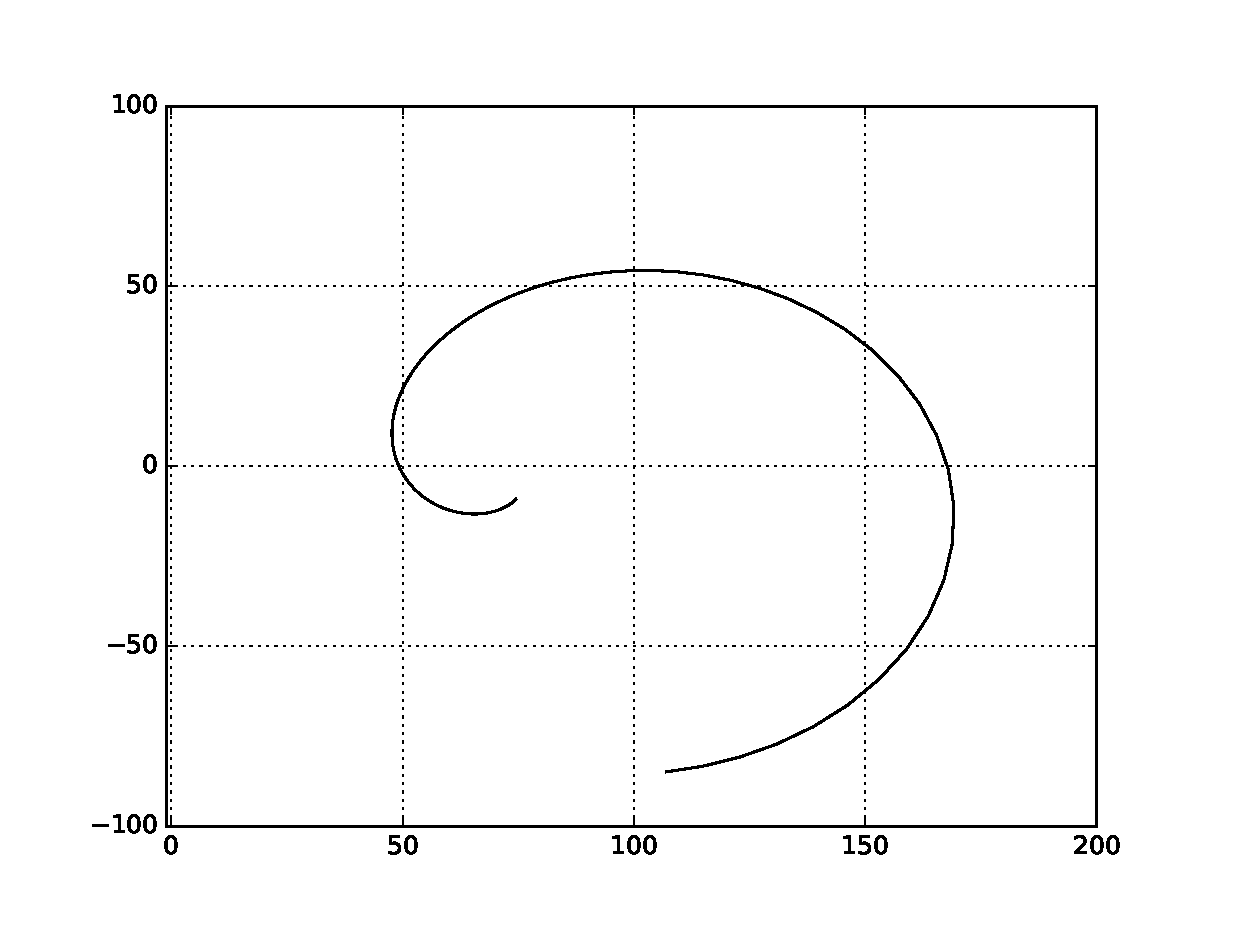
\includegraphics[width=\textwidth]{impedance2.eps}
  \caption{The figure shows the imput impedance of the antenna from Section~\ref{sec:c} in the frequency range $\SI{900}{\mega\hertz}$ to $\SI{3.6}{\giga\hertz}$. The horizontal axis shows the real part of the antenna impedance ($\Re\{Z_{\text{antenna}}\}$) and the vertical axis shows the imaginary part of the antenna impedance ($\Im\{Z_{\text{antenna}}\}$).}
  \label{fig:imp2}
\end{figure}
The return loss and the VSWR can be seen in Figure~\ref{fig:ans2}.
\begin{figure}
  \centering
  \includegraphics[width=\textwidth]{Answers2.eps}
  \caption{The figure shows the return loss (left) and the standing wave ratio (right) for the antenna from Section~\ref{sec:c} in the frequency range $\SI{900}{\mega\hertz}$ to $\SI{3.6}{\giga\hertz}$.}
  \label{fig:ans2}
\end{figure}

\end{document}